\begin{ejercicio}
   \begin{enumerate}
    \item[(a)] Explica qué error hay en la siguiente afirmación: Si $R$ es una región en el tercer cuadrante, entonces $\displaystyle\iint_R f(x, y)\, dA$ es negativa.
    \item[(b)] Da un ejemplo de una función $f(x, y)$ y una región rectangular $R$ tal que las sumas de Riemann que se obtienen usando la esquina inferior izquierda de cada subrectángulo son una sobreestimación de la integral de la función.
\end{enumerate}
\end{ejercicio}

\begin{respuesta}
<<<<<<< HEAD
     \textbf{Integrantes involucrados: Diego Hernandez Vazquez, Daniela Crisel Cabrera Galindo}\\
     
     \textbf{Inciso a:}\\Esta afirmacion es incorrecta porque esta asumiendo que al ser negativos los intervalos de integracion entonces el valor de la integral sera negativo, lo cual no es cierto; pues el valor de nuestra integral dependera del signo de la funcion. Esto es porque aunque $x;y$ tengan coordenadas negativas, el area de cada subrectangulo siempre sera positiva.\\
          \textit{Contrajemplo:} Buscamos una funcion simple tal que cuando $x<0$ y $y<0$ el resultado es positivo.\\
          Sea $$\int_{-2}^{-1} \int_{-2}^{-1} (x^2 + y^2)\, dx\, dy$$
          \begin{enumerate}
               \item Integramos respecto a $x$ ($y$ es constante)\\ $$\int_{-2}^{-1} \int_{-2}^{-1} (\frac{x^3}{3} + xy^2)\, dy$$
               \item Evaluando los limites de integracion $x_i = -2; x_s = -1$\\
               $$\left[\left(\frac{(-1)^3}{3} - y^2\right) - \left(\frac{(-2)^3}{3} - 2y^2\right)\right]$$\\
               $ = -\frac{1}{3} - y^2 + \frac{8}{3} + 2y^2 = \frac{7}{3} + y^2$ 
               \item Integramos respecto a $y$\\ 
               $\int_{-2}^{-1} (y^2 + \frac{7}{3})\, dy$\\  
               $= \frac{y^3}{3} + \frac{7}{3}y$ 
               \item Evaluando los limites de integracion $y_i=-2; y_s= -1$\\
               $$\left[\left(\frac{(-1)^3}{3} - \frac{7}{3}\right) - \left(\frac{(-2)^3}{3} + \frac{7}{3}\times -2\right)\right]$$\\
               $\frac{7}{3} + \frac{7}{3} = \frac{14}{3} > 0$
          \end{enumerate}
     
     \textbf{Inciso b:}\\Los subrectangulos de la superficie son de la forma $[x_{i-1},x_i] \times [y_{j-1},y_j]$
     el valor mas alto de la funcion sera donde $x;y$ sean lo mas pequenos posibles, es decir; la esquina inferior izquierda. En la siguiente imagen se muestra esta idea con mayor claridad
     \begin{figure}[H]
          \centering
          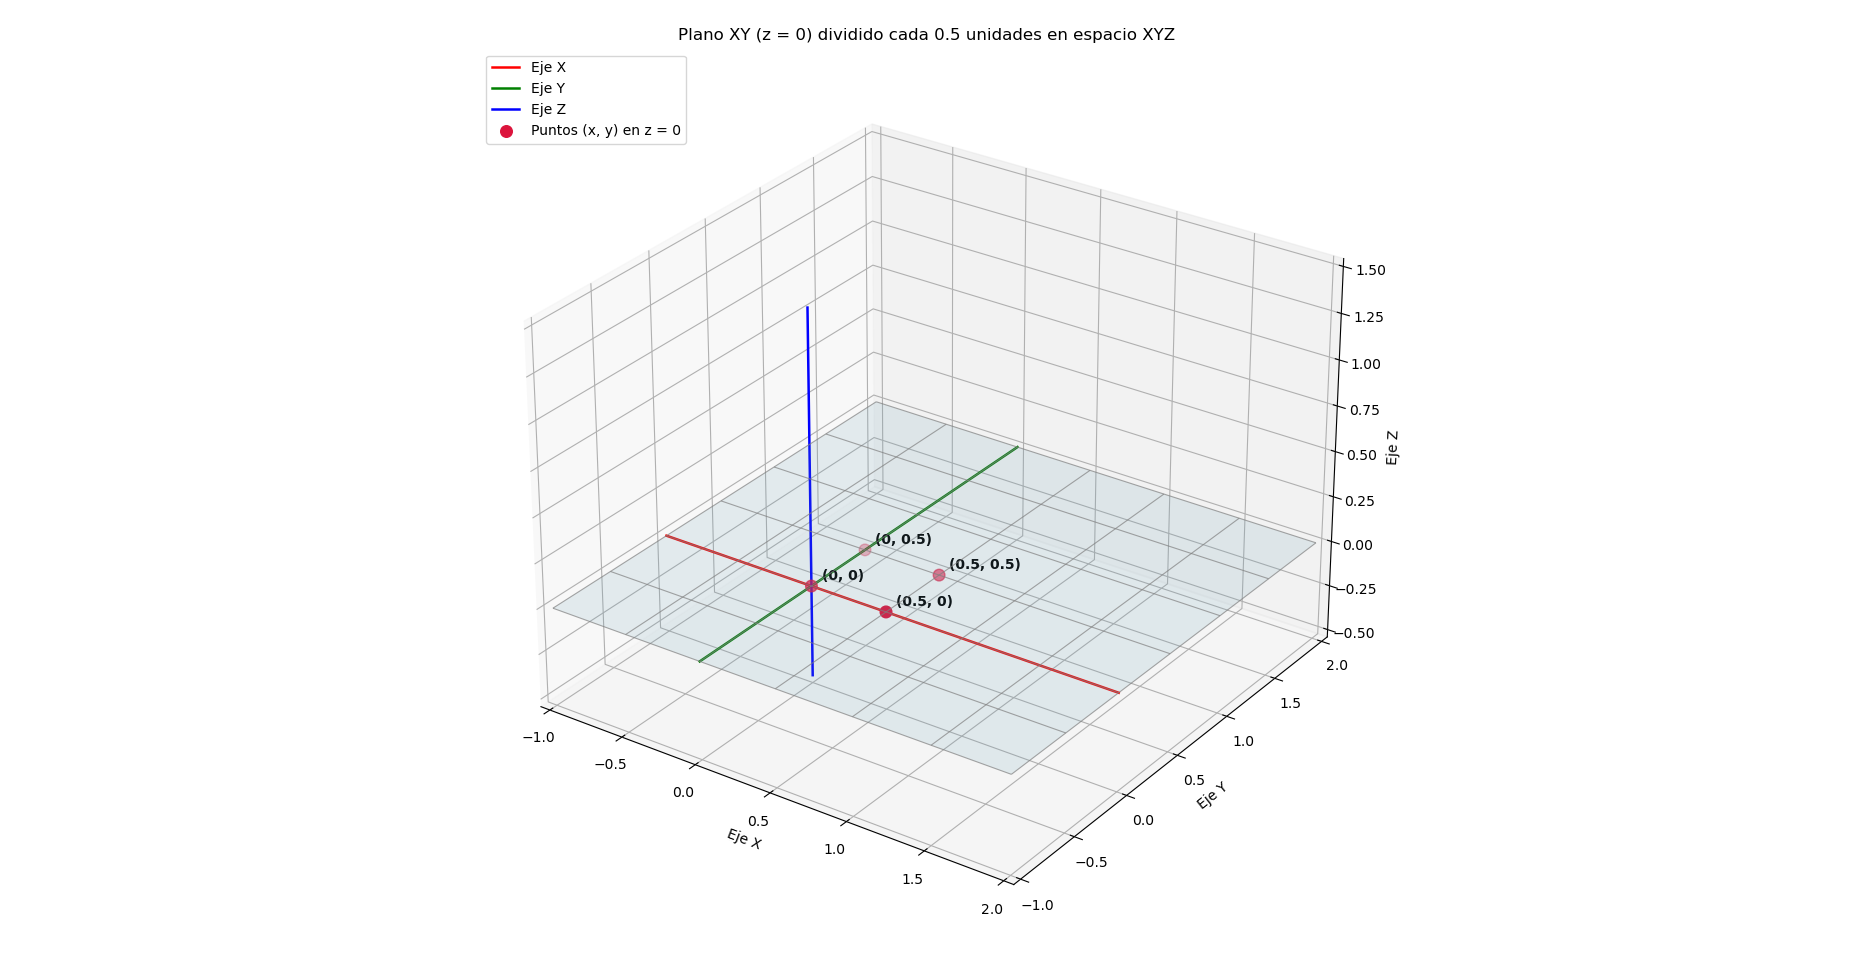
\includegraphics[width=0.8\textwidth]{Graficas.png}
    \caption{Subrectangulos en el plano xy}
     \end{figure}
     Ademas, para resolver el ejercicio hacemos uso de la siguiente propiedad:\\
     \textit{Propiedad: Para cualquier punto (x,y) dentro de un subrectangulo se cumple que $x \geq x_{i-1};y \geq y_{j-1}$  }\\
     Por lo que la funcion que elijamos debe ser decreciente en $x$ y en $y$\\De este modo tenemos que:\\
     Sea $f(x,y)= 4 - x - y$ \\ $$\frac{\partial f}{\partial x}=-1$$ $$\frac{\partial f}{\partial y}=-1$$\\
     Como $-1 < 0$ esto significa que si $x$ y $y$ aumentan la funcion disminuye.\\
     Por lo tanto, no importa que region $R$ elijamos del plano, en cualquier subrectangulo $[x_{i-1},x_i] \times [y_{j-1},y_j]$ el valor mas alto de la funcion siempre sera donde $x$ y $y$
     sean lo mas pequenos posibles, es decir deben ser de la forma $(x_{i-1}.y_{j-1})$\\
     Usando la propiedad\\
     $4 - x_{i-1} - y{j-1} \geq 4-x-y$\\
     $f(x_{i-1},y_{j-1}) \geq f(x,y)$\\
     
     Sea $R$ la region rectangular tal que $R = [0,1] \times [0,1]$ veremos que la suma de Rieman es mayor que la integral de la funcion.\\
     \textbf{Suma de Riemann}\\
     Sea $n=2$ los subintervalos en los que se divide la region y $[0,1]$ un intervalo en $x$ y $y$\\
     $\Delta x= \frac{b-a}{n} = \frac{1-0}{2}=\frac{1}{2} $\\
     $\Delta y= \frac{b-a}{n} = \frac{1-0}{2}=\frac{1}{2} $\\
     $\Delta A =(0.5)(0.5)= 0.25$\\
     \textit{Punto muestra: Tomamos las esquinas inferiores izquierdas}\\
     \begin{itemize}
          \item $(0,0) \longrightarrow f(0,0) = 4$
          \item $(0.5,0) \longrightarrow f(0.5,0) = 3.5$
          \item $(0,0.5) \longrightarrow f(0,0.5) = 3.5$
          \item $(0.5,0.5) \longrightarrow f(0.5,0.5) = 3$
     \end{itemize}
     $$\sum_{i=1}^{n} f(x_i^*)\,\Delta A$$\\
     $ = [f(0,0) + f(0.5,0) + f(0,0.5) + f(0.5,0.5)] \cdot 0.25 $\\
     $=(4 + 3.5 + 3.5 + 3) \cdot 0.25$\\
     $=3.5$\\
     \textbf{Integral de la funcion}\\
     \textit{Integrando con respecto a x}\\
     $$\int_{1}^{0} \int_{1}^{0} (4-x-y)\, dx\, dy$$
     $$\int_{1}^{0} (4x - \frac{x^2}{2} -xy) dy$$\\
     $\Longrightarrow[(4)(1) - \frac{1}{2} - y] - [(4)(0) - \frac{0}{2} - 0]$\\
     $4 - \frac{1}{2}-y - 0 = \frac{7}{2} - y$\\
     \textit{Integrando con respecto a y}\\
     $$\int_{1}^{0} \frac{7}{2} - y dy$$\\
     $ \longrightarrow [\frac{7}{2} - \frac{1}{2}] - [0-0]$\\
     $ = \frac{6}{2} = 3$\\
     Como $3.5 > 3$ entonces quedo comprobado para nuestro ejemplo que la suma de Riemann es una sobreestimacion de la integral
\end{respuesta}
=======

     \textbf{Integrantes involucrados: Diego Hernandez Vazquez,}
\end{respuesta}
>>>>>>> fe700d12d8d1e2bcb6715829e2cb203286a448c7
